\chapter{Resultados usando el Modelo 2\\
(Faster R-CNN)}

En esta sección se presentan los resultados obtenidos al usar el modelo 2. En este modelo se implementa la técnica de detección de objetos usando la red pre-entrenad Faster R-CNN (ver sección \ref{sec:Faster}).  Primero  se  presentan  los  resultados  del  modelo  1  usando  la  base  de datos \textit{CharsBoxPlateCol}. Luego, se muestran los resultados realizando aumento de datos con la aplicación RoboFlow (ver sección \ref{sec:basedatos3}). Finalmente se compara el Modelo 2 con el modelo 1.

El sistema de reconocimiento completo funciona de la siguiente manera: 
\begin{itemize}
    
    \item[i] Ingresa al sistema la imagen del auto que contiene la placa a ser reconocida, tal como se muestra en la figura \ref{fig:Cargamos imagen deteccion}.

\begin{figure}[H]
\centering
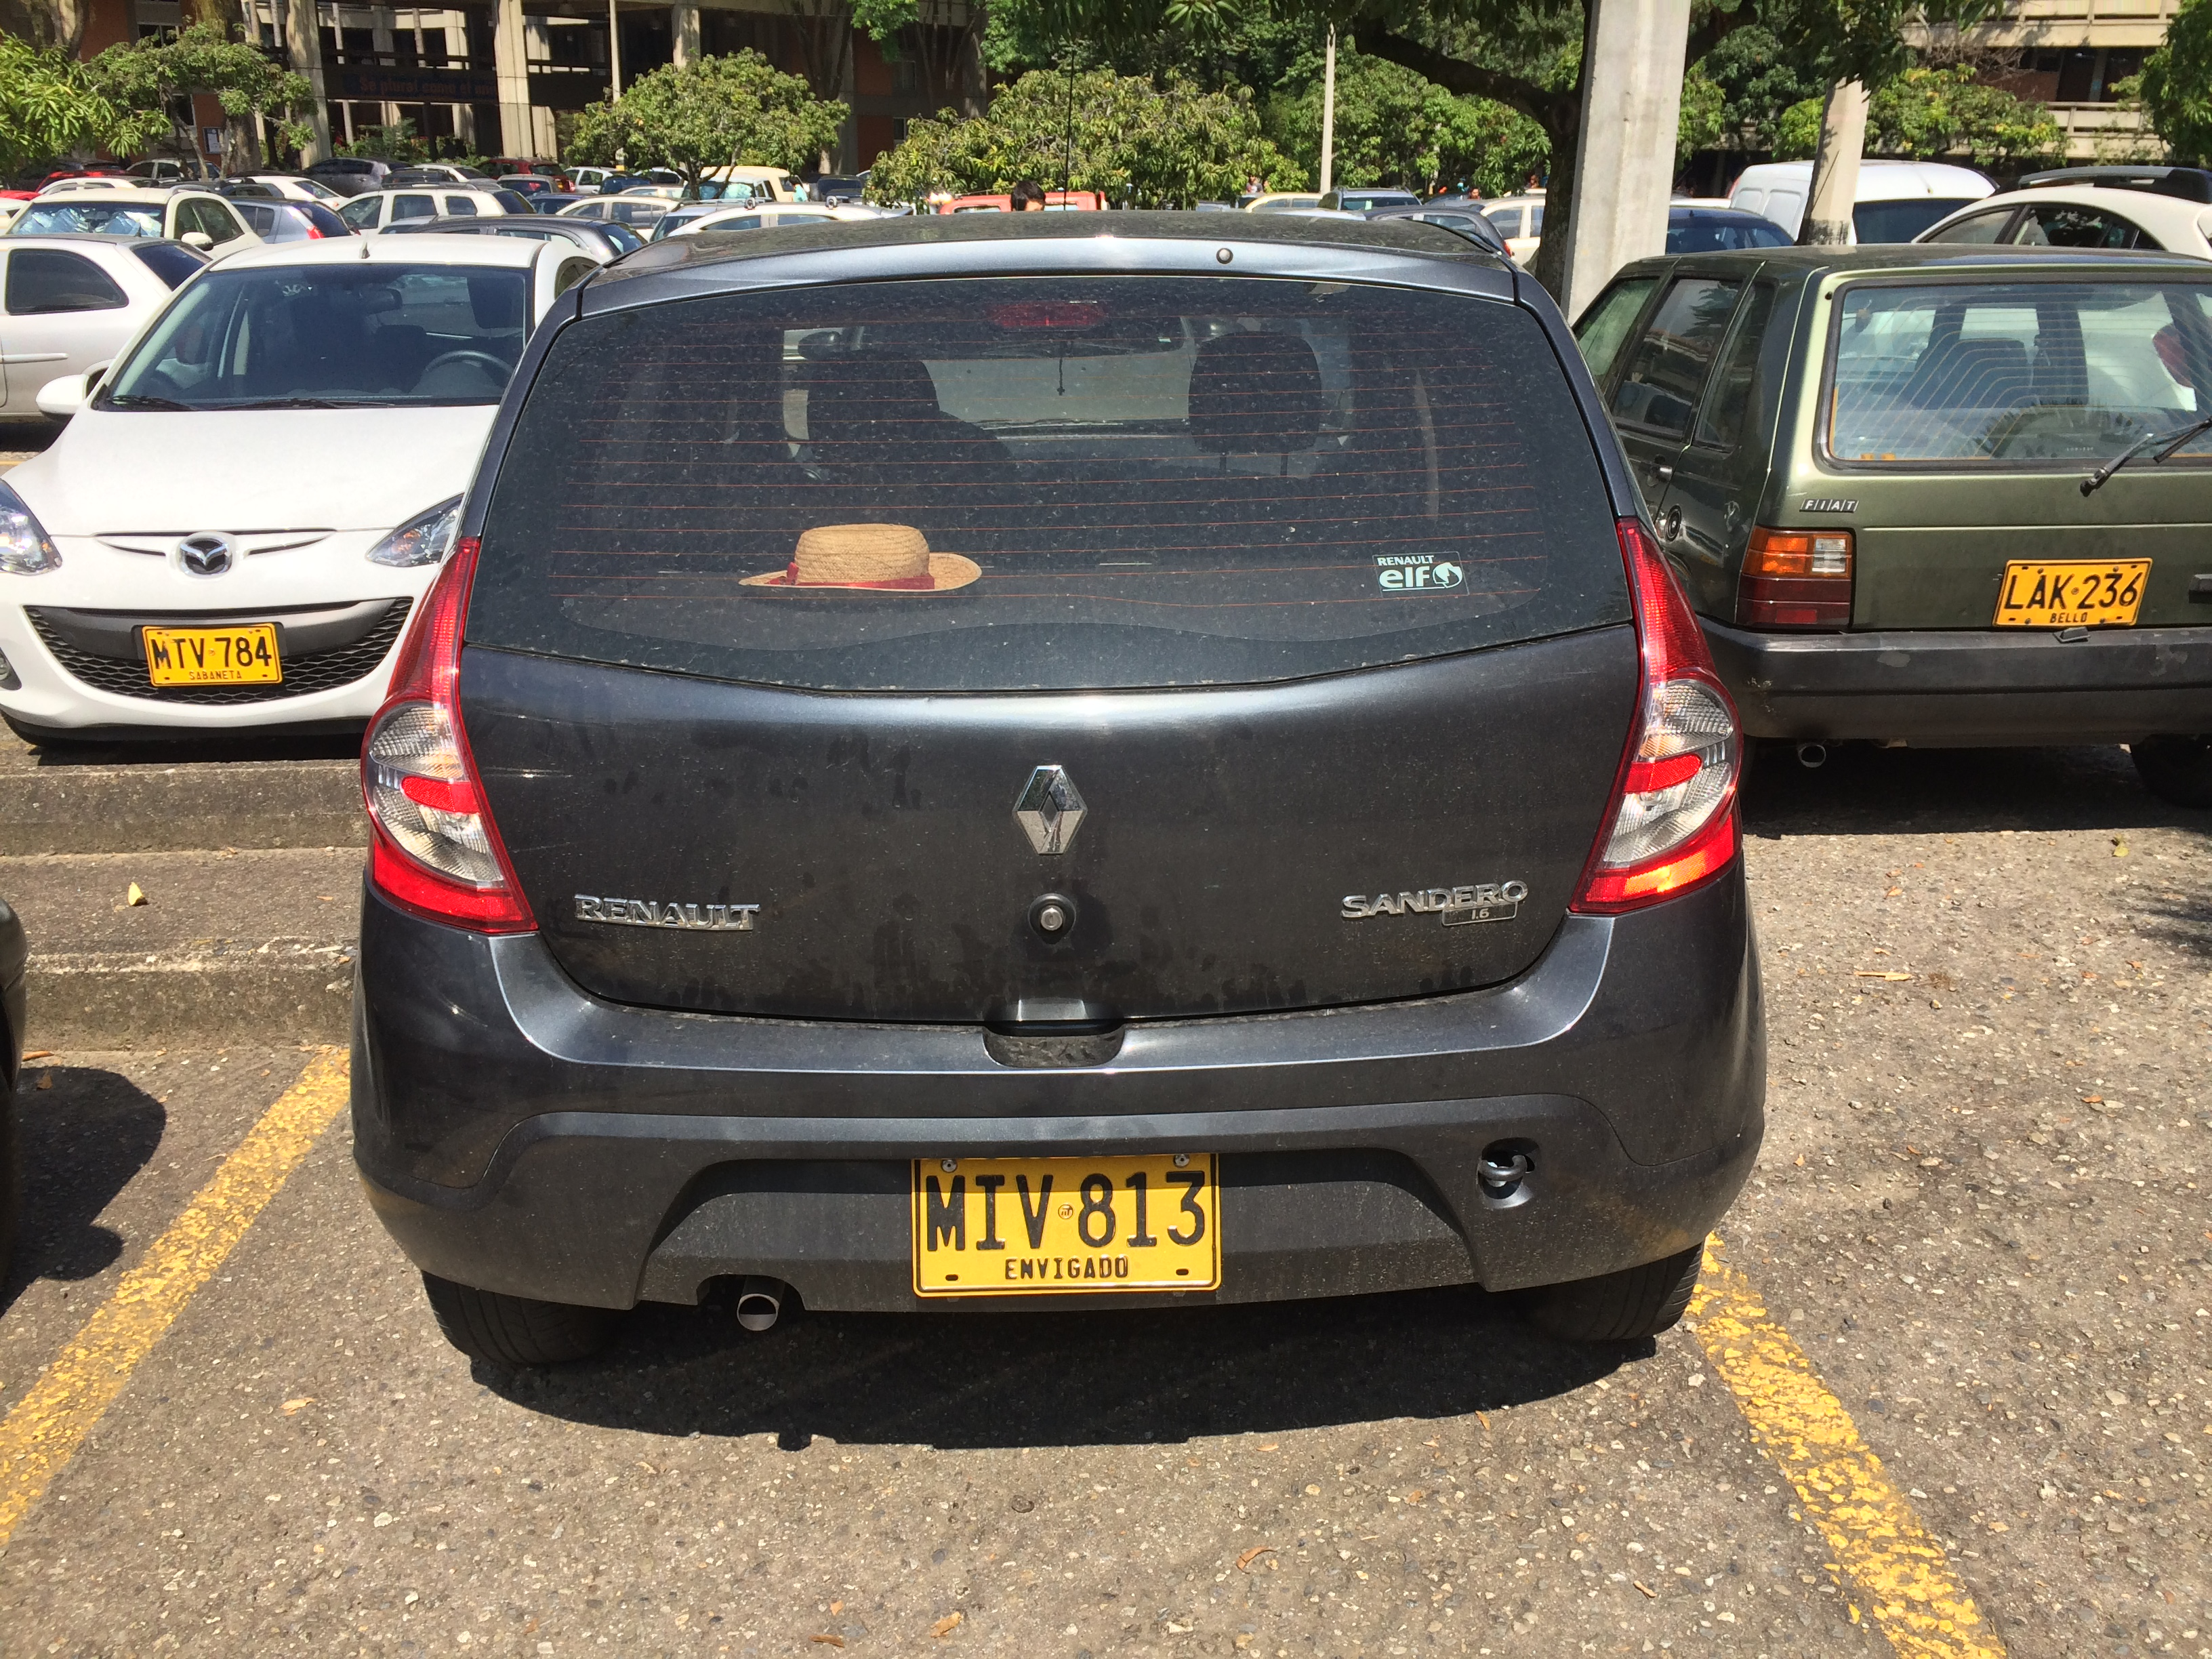
\includegraphics[width=0.6\linewidth]{imagenes/RESULTADOS/carro_detec.JPG}
\caption{Imagen de entrada al sistema}
\label{fig:Cargamos imagen deteccion}
\end{figure}

\item[ii] Se realiza una segmentación de la placa, tal como se puede observar en la figura \ref{fig:Placa segmentada}.

\item[iii] Finalmente, la placa segmentada entra al modelo 2, Faster R-CNN, ya entrenado. El resultado se puede observar en la figura \ref{fig:caracteres detectados}. Allí se puede observar el cuadro que delimita la región donde el sistema detectó que había un caracter y encima de cada cuadro el nombre de la clase detectado, con su respectivo porcentaje de confianza en la detección. La tabla \ref{tab:Porcentaje de reconocimiento} muestra los resultados obtenidos para el ejemplo en consideración. Para tal caso, el sistema detecta que hay 6 caracteres y todos los etiqueta correctamente. Sin embargo, aunque el sistema los reconoce todos correctamente, cada uno de ellos tiene una confiabilidad en el reconocimiento diferente. Es posible que en algunos casos detecte un caracter correctamente pero con un porcentaje de confiabilidad muy bajo (Letra M en el ejemplo), en otros puede que lo detecte pero no lo etiquete correctamente y en otros que ni siquiera detecte el caracter. 
\end{itemize}

\begin{figure}[H]
\centering
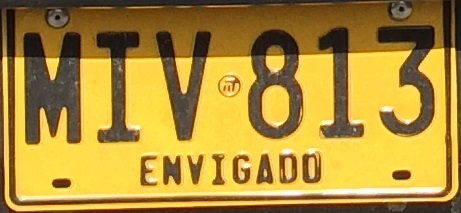
\includegraphics[width=0.5\linewidth]{imagenes/RESULTADOS/placa_carro_detec.JPG}
\caption{Placa segmentada}
\label{fig:Placa segmentada}
\end{figure}

\begin{figure}[H]
\centering
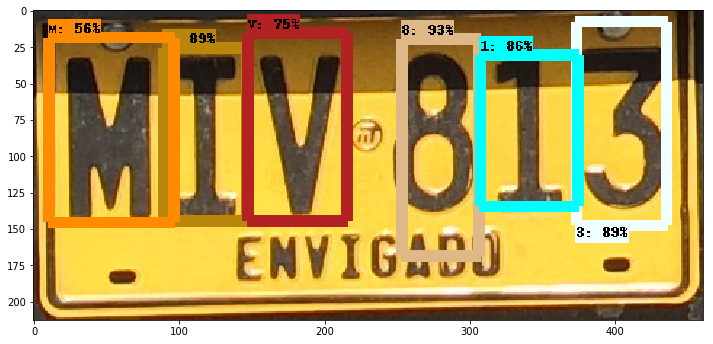
\includegraphics[width=0.5\linewidth]{imagenes/MODELO_5/resul_3_mod5.png}
\caption{caracteres detectados}
\label{fig:caracteres detectados}
\end{figure}

%La figura \ref{fig:Cargamos imagen deteccion} es la imagen de entrada a nuestro sistema de reconocimiento, luego de la segmentación de la placa, figura \ref{fig:Placa segmentada}, hacemos el proceso de detección de caracteres con el modelo entrenado con la data  \textit{CharsBoxPlateCol} y obtenemos los resultados de la figura \ref{fig:caracteres detectados}, donde los porcentajes en los cuadros delimitadores me indican el nivel de confiabilidad de cada caracter detectado y la clase a la cual pertenece. En la tabla \ref{tab:Porcentaje de reconocimiento} la primera columna indica el caracter real de la placa, la segunda columna el caracter detectado por el modelo y la tercera columna el porcentaje de confiabilidad al detectar el caracter. En este caso se logró reconocer los 6 caracteres con los siguientes porcentajes

\begin{table}[H]
    \centering
    \resizebox{\textwidth}{!}{
    \begin{tabular}{|c|c|c|}
    \hline
         Caracter de entrada & Caracter detectado & Porcentaje de reconocimiento  \\ \hline
         Letra M & Letra M & 56\% \\ \hline
         Letra I & Letra I & 89\% \\ \hline
         Letra V & Letra V & 75\% \\ \hline
         Número 8 & Número 8 & 93\% \\ \hline
         Número 1 & Número 1 & 86\% \\ \hline
         Número 3 & Número 3 & 89\% \\ \hline
    \end{tabular}
    }
    \caption{Detección de caracteres con porcentajes de acierto}
    \label{tab:Porcentaje de reconocimiento}
\end{table}



%=================================
\section{Resultado usando la base de datos \textit{CharsBoxPlateCol}}
%================================
%Es importante resaltar que todo este proceso de entrenamiento se realizó en google colaboratory y en el test que se realizó con 3 placas, se detectaron los 18 caracteres sin inconvenientes, con 2 porcentajes de certeza bajos de 68\% y 75\% los demás oscilan entre 88\% y 98\%. La figura \ref{fig:faster} es una muestra de dos placas con la detección de los caracteres por medio de la \textbf{Faster R-CNN}, independiente de su grado de inclinación, la detección fue muy positiva, ya que reconoció todos los 6 caracteres en cada placa.

Presentamos ahora los resultados del modelo 2 usando para el entrenamiento la base de datos \textit{CharsBoxPlateCol}. El entrenamiento también se realizó en Google Colaboratory. El test fue realizado con 32 imágenes de placas colombianas, que corresponden a 192 caracteres a reconocer. Estas placas las clasificaremos como placa SI reconocida y  placa NO reconocida, a partir de un porcentaje umbral de confiabilidad del 60\%. Así, todo caracter con un porcentaje inferior a este valor, se considera caracter no reconocido, e indica que la placa en general tampoco lo es. Si el modelo nos muestra dos cuadros delimitadores en un mismo caracter, es escogido aquel con mayor porcentaje de acierto, sea correcto o incorrecto el resultado.

\begin{comment}
    \begin{figure}[H]
\centering
  \subfigure[]{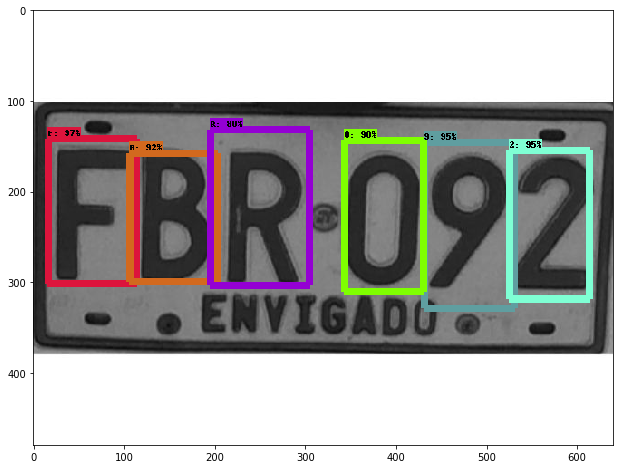
\includegraphics[width=0.4\textwidth]{imagenes/MODELO_5/resul_1_mod5.png}}
    \subfigure[]{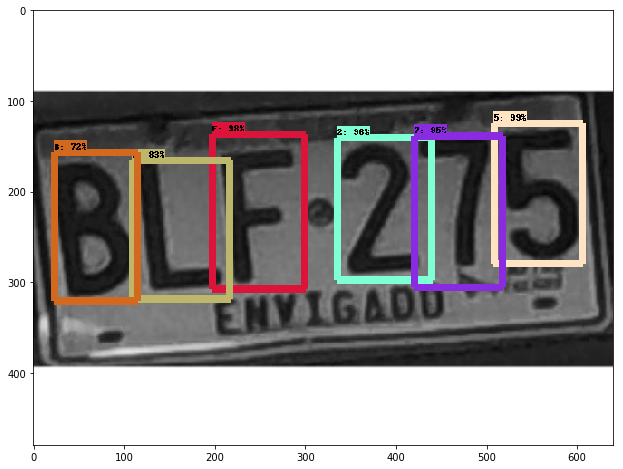
\includegraphics[width=0.4\textwidth]{imagenes/MODELO_5/resul_2_mod5.png}}
    \caption{Resultado de la detección de caracteres por medio de una Faster R-CNN }
    \label{fig:faster}  
\end{figure}
\end{comment}

A continuación se muestran los resultado obtenidos al detectar los caracteres en 32 placas colombianas:

\subsection{Placas detectadas y reconocidas acertadamente}

A continuación presentamos los resultados en los cuales el Modelo 2 detectó todos los caracteres y los reconoció acertadamente con un porcentaje mayor al 60\%.  
% PLACA 1

\begin{figure}[H]
\centering
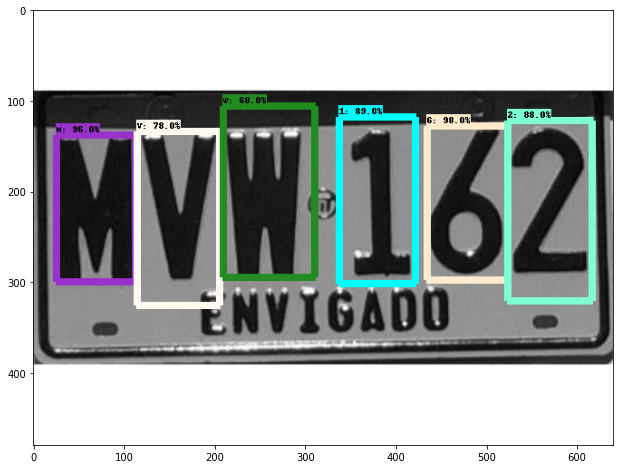
\includegraphics[width=0.4\linewidth]{imagenes/caracteres detectados/1.png}
\caption{Placa 1}
\label{fig:caracteres detectados p1}
\end{figure}

\begin{table}[H]
    \centering
    \resizebox{\textwidth}{!}{
    \begin{tabular}{||c|c|c||}
    \hline \hline
         Caracter Placa & Caracter detectado & Porcentaje de reconocimiento 
         \\ \hline \hline
         Letra M & Letra M & 90\%   \\ \cline{1-3}
         Letra V & Letra V & 78\%  \\ \cline{1-3}
         Letra W & Letra W & 68\% \\ \cline{1-3}
         Número 1 & Número 1 & 89\%  \\ \cline{1-3}
         Número 6 & Número 6 & 98\%  \\ \cline{1-3}
         Número 2 & Número 2 & 88\%  \\ \hline \hline
    \end{tabular}
    }
    \caption{Detección de caracteres con porcentajes de acierto placa 1}
    \label{tab:p1}
\end{table}

% PLACA 2
\begin{figure}[H]
\centering
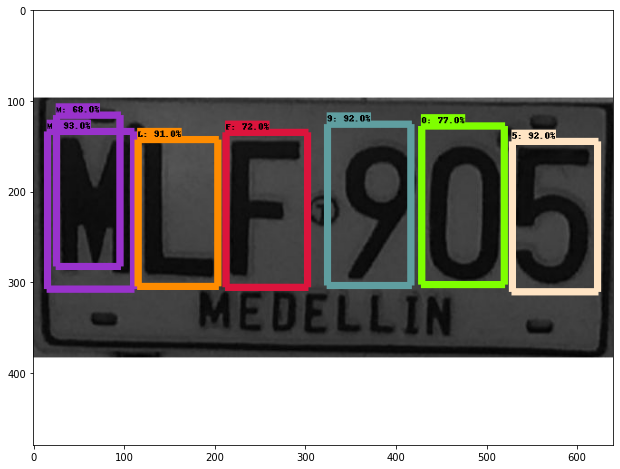
\includegraphics[width=0.4\linewidth]{imagenes/caracteres detectados/2.png}
\caption{Placa 2}
\label{fig:caracteres detectados p2}
\end{figure}

\begin{table}[H]
    \centering
    \resizebox{\textwidth}{!}{
    \begin{tabular}{||c|c|c||}
    \hline \hline
         Caracter Placa & Caracter detectado & Porcentaje de reconocimiento 
         l  \\ \hline \hline
         Letra M & Letra M & 93\% \\ \cline{1-3}
         Letra L & Letra L & 91\%  \\ \cline{1-3}
         Letra F & Letra F & 72\%  \\ \cline{1-3}
         Número 9 & Número 9 & 92\% \\ \cline{1-3}
         Número 0 & Número 0 & 77\% \\ \cline{1-3}
         Número 5 & Número 5 & 92\% \\ \hline \hline
    \end{tabular}
    }
    \caption{Detección de caracteres con porcentajes de acierto placa 2}
    \label{tab:p2}
\end{table}

% PLACA 3------------
\begin{figure}[H]
\centering
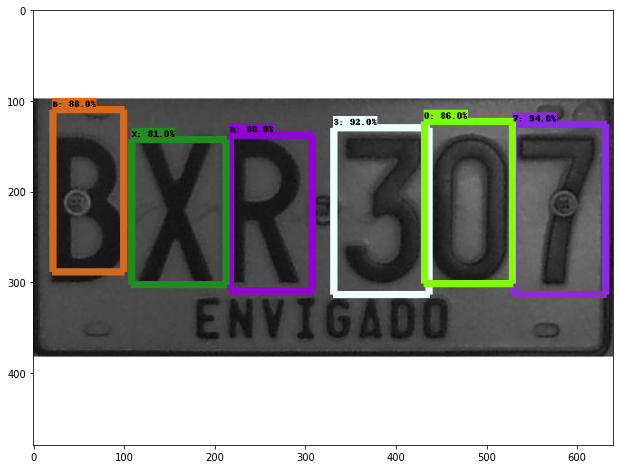
\includegraphics[width=0.4\linewidth]{imagenes/caracteres detectados/nuevo entrenamiento/16.png}
\caption{Placa 3}
\label{fig:caracteres detectados p3}
\end{figure}

\begin{table}[H]
    \centering
    \resizebox{\textwidth}{!}{
    \begin{tabular}{||c|c|c||}
    \hline \hline
         Caracter Placa & Caracter detectado & Porcentaje de reconocimiento 
         \\  \hline \hline
         Letra B & Letra B & 93\%  \\ \cline{1-3}
         Letra X & Letra X & 93\%  \\ \cline{1-3}
         Letra R & Letra R & 74\%  \\ \cline{1-3}
         Número 3 & Número 3 & 98\%  \\ \cline{1-3}
         Número 0 & Número 0 & 79\%  \\ \cline{1-3}
         Número 7 & Número 7 & 80\%  \\ \hline \hline
    \end{tabular}
    }
    \caption{Detección de caracteres con porcentajes de acierto placa 3}
    \label{tab:p3}
\end{table}



% PLACA 4-----------
\begin{figure}[H]
\centering
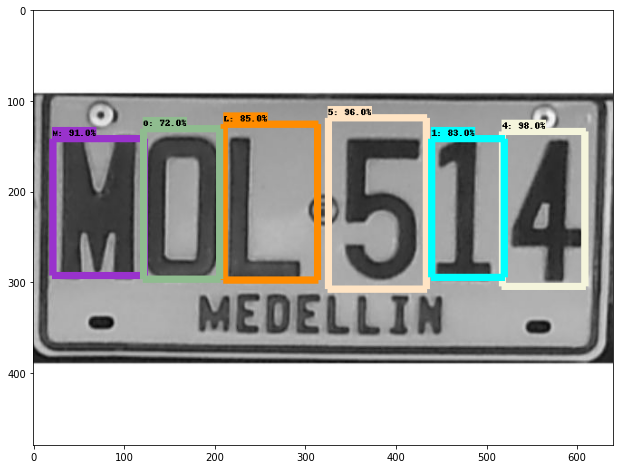
\includegraphics[width=0.4\linewidth]{imagenes/caracteres detectados/5.png}
\caption{Placa 4}
\label{fig:caracteres detectados p5}
\end{figure}

\begin{table}[H]
    \centering
    \resizebox{\textwidth}{!}{
    \begin{tabular}{||c|c|c||}
    \hline \hline
         Caracter Placa & Caracter detectado & Porcentaje de reconocimiento 
         \\  \hline \hline
         Letra M & Letra M & 91\% \\ \cline{1-3}
         Letra O & Letra O & 72\% \\ \cline{1-3}
         Letra L & Letra L & 85\% \\ \cline{1-3}
         Número 5 & Número 5 & 96\%  \\ \cline{1-3}
         Número 1 & Número 1 & 83\%  \\ \cline{1-3}
         Número 4 & Número 4 & 98\%  \\ \hline \hline
    \end{tabular}
    }
    \caption{Detección de caracteres con porcentajes de acierto placa 4}
    \label{tab:p5}
\end{table}


% PLACA 5------------
\begin{figure}[H]
\centering
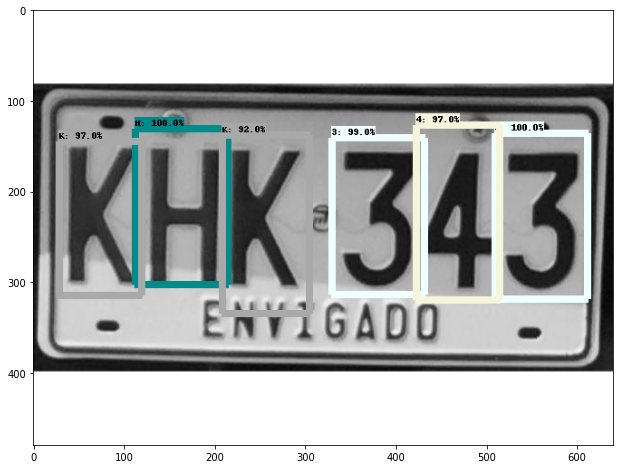
\includegraphics[width=0.4\linewidth]{imagenes/caracteres detectados/nuevo entrenamiento/25.png}
\caption{Placa 5}
\label{fig:caracteres detectados p6}
\end{figure}

\begin{table}[H]
    \centering
  \resizebox{\textwidth}{!}{
    \begin{tabular}{||c|c|c||}
    \hline \hline
         Caracter Placa & Caracter detectado & Porcentaje de reconocimiento 
         \\  \hline \hline
         Letra K & Letra K & 97\%  \\ \cline{1-3}
         Letra H & Letra H & 100\% \\ \cline{1-3}
         Letra K & Letra K & 92\%  \\ \cline{1-3}
         Número 3 & Número 3  & 99\% \\ \cline{1-3}
         Número 4 & Número 4 & 97\%  \\ \cline{1-3}
         Número 3 & Número 3 & 100\% \\ \hline \hline
    \end{tabular}
    }
    \caption{Detección de caracteres con porcentajes de acierto placa 5}
    \label{tab:p6}
\end{table}

% PLACA 6----------

\begin{figure}[H]
\centering
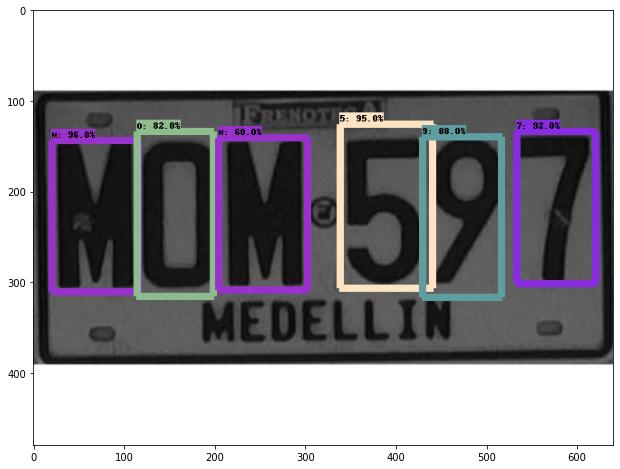
\includegraphics[width=0.4\linewidth]{imagenes/caracteres detectados/7.png}
\caption{Placa 6}
\label{fig:caracteres detectados p7}
\end{figure}

\begin{table}[H]
    \centering
    \resizebox{\textwidth}{!}{
    \begin{tabular}{||c|c|c||c||}
    \hline \hline
         Caracter Placa & Caracter detectado & Porcentaje de reconocimiento 
         \\  \hline \hline
         Letra M & Letra M & 96\%  \\ \cline{1-3}
         Letra O & Letra O & 82\%  \\ \cline{1-3}
         Letra M & Letra M & 60\%  \\ \cline{1-3}
         Número 5 & Número 5 & 95\% \\ \cline{1-3}
         Número 9 & Número 9 & 88\% \\ \cline{1-3}
         Número 7 & Número 7 & 92\% \\ \hline
         \hline
         \end{tabular}
    }
    \caption{Detección de caracteres con porcentajes de acierto placa 6}
    \label{tab:p7}
\end{table}

% PLACA 7------------

\begin{figure}[H]
\centering
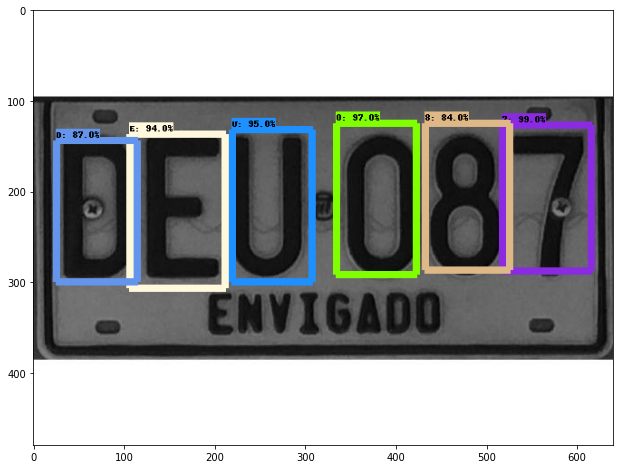
\includegraphics[width=0.4\linewidth]{imagenes/caracteres detectados/nuevo entrenamiento/21.png}
\caption{Placa 7}
\label{fig:caracteres detectados p8}
\end{figure}

\begin{table}[H]
    \centering
    \resizebox{\textwidth}{!}{
    \begin{tabular}{||c|c|c||}
    \hline \hline
         Caracter Placa & Caracter detectado & Porcentaje de reconocimiento
         \\  \hline \hline
         Letra D & Letra D & 87\%  \\ \cline{1-3}
         Letra E & Letra E & 94\%  \\ \cline{1-3}
         Letra U & Letra U & 95\% \\\cline{1-3}
         Número 0 & Número 0 & 97\%  \\ \cline{1-3}
         Número 8 & Número 8 & 84\%  \\ \cline{1-3}
         Número 7 & Número 7 & 99\% \\ \hline \hline
    \end{tabular}
    }
    \caption{Detección de caracteres con porcentajes de acierto placa 7}
    \label{tab:p8}
\end{table}

% PLACA 8-----------

\begin{figure}[H]
\centering
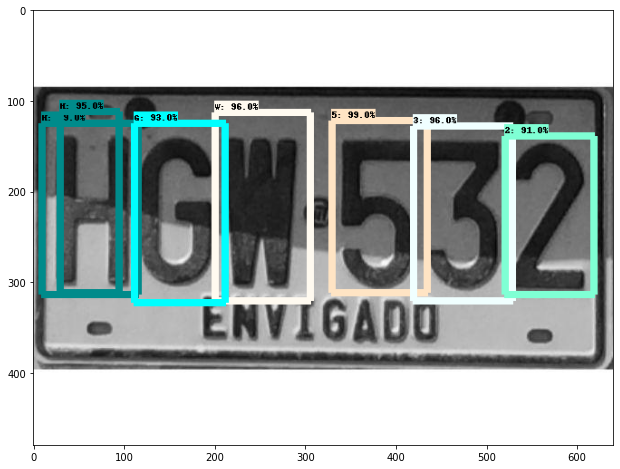
\includegraphics[width=0.4\linewidth]{imagenes/caracteres detectados/nuevo entrenamiento/2.png}
\caption{Placa 8}
\label{fig:caracteres detectados p9}
\end{figure}

\begin{table}[H]
    \centering
    \resizebox{\textwidth}{!}{
    \begin{tabular}{||c|c|c||}
    \hline \hline
         Caracter Placa & Caracter detectado & Porcentaje de reconocimiento 
         \\  \hline \hline
         Letra H & Letra H & 95\%  \\ \cline{1-3}
         Letra G & Letra G & 93\%  \\ \cline{1-3}
         Letra W & Letra W & 96\%  \\ \cline{1-3}
         Número 5 & Número 5 & 99\%  \\ \cline{1-3}
         Número 3 & Número 3 & 96\% \\ \cline{1-3}
         Número 2 & Número 2 & 91\% \\ \hline
         \hline
         \end{tabular}
    }
    \caption{Detección de caracteres con porcentajes de acierto placa 8}
    \label{tab:p9}
\end{table}


% PLACA 9------------

\begin{figure}[H]
\centering
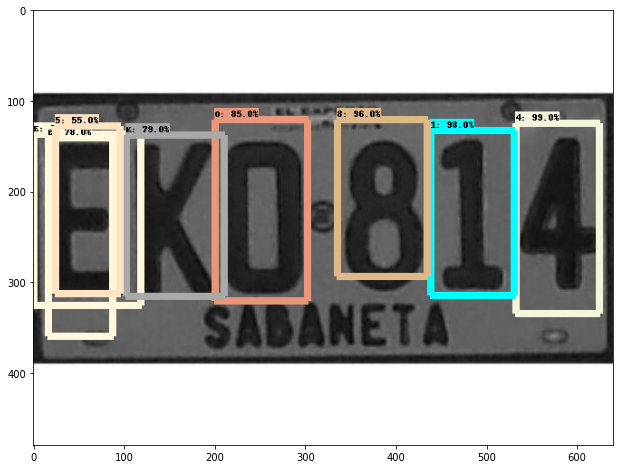
\includegraphics[width=0.4\linewidth]{imagenes/caracteres detectados/nuevo entrenamiento/29.png}
\caption{Placa 9}
\label{fig:caracteres detectados p10}
\end{figure}

\begin{table}[H]
    \centering
    \resizebox{\textwidth}{!}{
    \begin{tabular}{||c|c|c||}
    \hline \hline
         Caracter Placa & Caracter detectado & Porcentaje de reconocimiento 
         \\  \hline \hline
         Letra E & Letra E & 78\%  \\ \cline{1-3}
         Letra K & Letra K & 79\%  \\ \cline{1-3}
         Letra O & Letra O & 85\%  \\ \cline{1-3}
         Número 8 & Número 8 & 96\% \\ \cline{1-3}
         Número 1 & Número 1 & 98\% \\ \cline{1-3}
         Número 4 & Número 4 & 99\% \\ \hline
         \hline
         \end{tabular}
    }
    \caption{Detección de caracteres con porcentajes de acierto placa 9}
    \label{tab:p10}
\end{table}



% PLACA 10-----------
\begin{figure}[H]
\centering
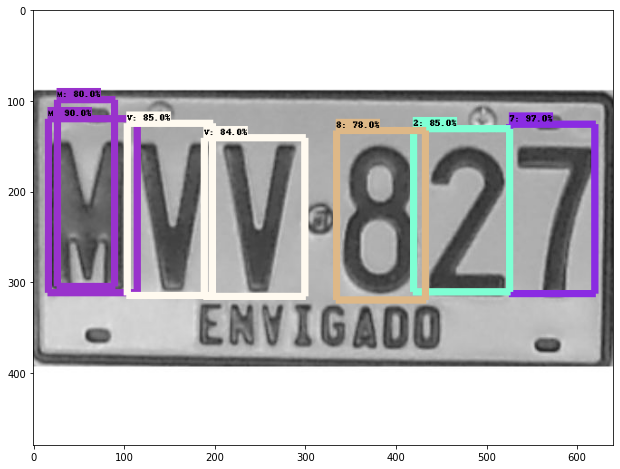
\includegraphics[width=0.4\linewidth]{imagenes/caracteres detectados/11.png}
\caption{Placa 10}
\label{fig:caracteres detectados p11}
\end{figure}

\begin{table}[H]
    \centering
    \resizebox{\textwidth}{!}{
    \begin{tabular}{||c|c|c||}
    \hline \hline
         Caracter Placa & Caracter detectado & Porcentaje de reconocimiento \\  \hline \hline
         Letra M & Letra M & 90\%  \\ \cline{1-3}
         Letra V & Letra V & 85\%  \\ \cline{1-3}
         Letra V & Letra V & 84\%  \\ \cline{1-3}
         Número 8 & Número 8 & 78\%  \\ \cline{1-3}
         Número 2 & Número 2 & 85\%  \\ \cline{1-3}
         Número 7 & Número 7 & 97\% \\ \hline
         \hline
         \end{tabular}
    }
    \caption{Detección de caracteres con porcentajes de acierto placa 10}
    \label{tab:p11}
\end{table}




% PLACA 11------------
\begin{figure}[H]
\centering
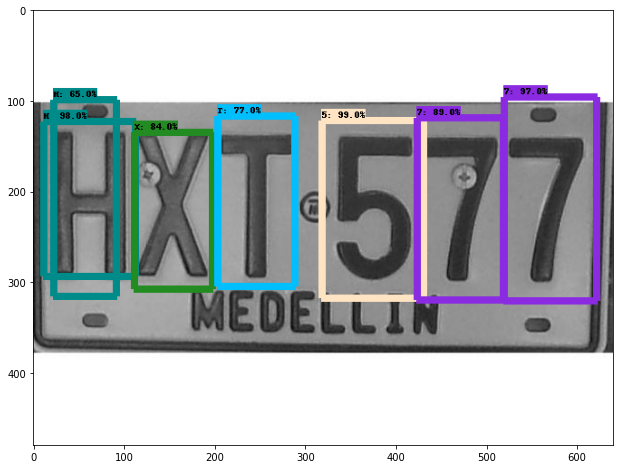
\includegraphics[width=0.4\linewidth]{imagenes/caracteres detectados/nuevo entrenamiento/3.png}
\caption{Placa 11}
\label{fig:caracteres detectados p13}
\end{figure}

\begin{table}[H]
    \centering
    \resizebox{\textwidth}{!}{
    \begin{tabular}{||c|c|c||}
    \hline \hline
         Caracter Placa & Caracter detectado & Porcentaje de reconocimiento  \\  \hline \hline
         Letra H & Letra H & 98\%  \\ \cline{1-3}
         Letra X & Letra X & 84\%  \\ \cline{1-3}
         Letra T & Letra T & 77\%  \\ \cline{1-3}
         Número 5 & Número 5 & 99\%  \\ \cline{1-3}
         Número 7 & Número 7 & 89\%  \\ \cline{1-3}
         Número 7 & Número 7 & 97\% \\ \hline
         \hline
         \end{tabular}
    }
    \caption{Detección de caracteres con porcentajes de acierto placa 11}
    \label{tab:p13}
\end{table}

% PLACA 12-----------
\begin{figure}[H]
\centering
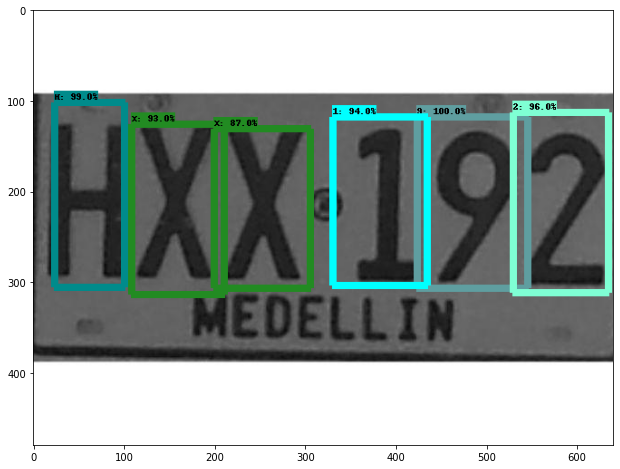
\includegraphics[width=0.4\linewidth]{imagenes/caracteres detectados/nuevo entrenamiento/28.png}
\caption{Placa 12}
\label{fig:caracteres detectados p14}
\end{figure}

\begin{table}[H]
    \centering
    \resizebox{\textwidth}{!}{
    \begin{tabular}{||c|c|c||}
    \hline \hline
         Caracter Placa & Caracter detectado & Porcentaje de reconocimiento \\  \hline \hline
         Letra H & Letra H & 99\%  \\ \cline{1-3}
         Letra X & Letra X & 93\%  \\ \cline{1-3}
         Letra T & Letra T & 87\%  \\ \cline{1-3}
         Número 1 & Número 1 & 94\%  \\ \cline{1-3}
         Número 9 & Número 9 & 100\%  \\ \cline{1-3}
         Número 2 & Número 2 & 96\% \\ \hline
         \hline
         \end{tabular}
    }
    \caption{Detección de caracteres con porcentajes de acierto placa 12}
    \label{tab:p14}
\end{table}

% PLACA 13------------
\begin{figure}[H]
\centering
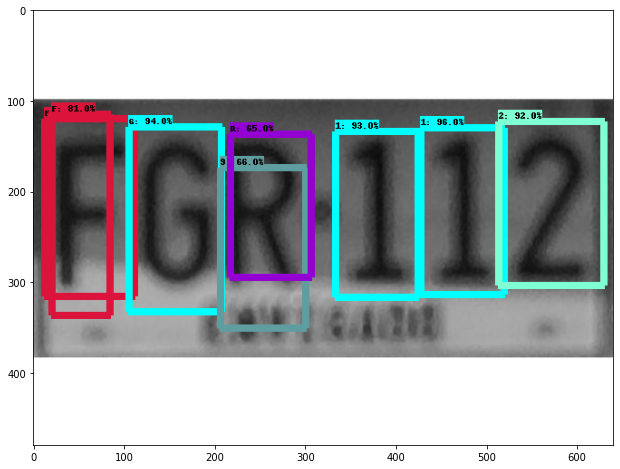
\includegraphics[width=0.4\linewidth]{imagenes/caracteres detectados/nuevo entrenamiento/30.png}
\caption{Placa 13}
\label{fig:caracteres detectados p15}
\end{figure}

\begin{table}[H]
    \centering
    \resizebox{\textwidth}{!}{
    \begin{tabular}{||c|c|c||}
    \hline \hline
         Caracter Placa & Caracter detectado & Porcentaje de reconocimiento  \\  \hline \hline
         Letra F & Letra F & 91\%  \\ \cline{1-3}
         Letra G & Letra G & 94\%  \\ \cline{1-3}
         Letra R & Letra R & 65\%  \\ \cline{1-3}
         Número 1 & Número 1 & 93\%  \\ \cline{1-3}
         Número 1 & Número 1 & 96\%  \\ \cline{1-3}
         Número 2 & Número 2 & 92\% \\ \hline
         \hline
         \end{tabular}
    }
    \caption{Detección de caracteres con porcentajes de acierto placa 13}
    \label{tab:p15}
\end{table}


% PLACA 14------------
\begin{figure}[H]
\centering
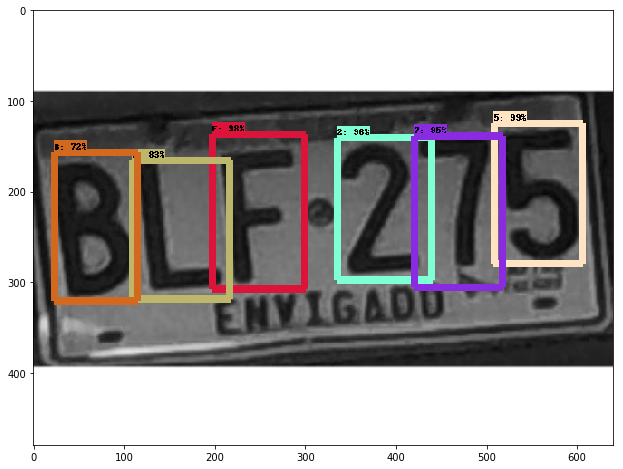
\includegraphics[width=0.4\linewidth]{imagenes/MODELO_5/resul_2_mod5.png}
\caption{Placa 13}
\label{fig:caracteres detectados p16}
\end{figure}

\begin{table}[H]
    \centering
    \resizebox{\textwidth}{!}{
    \begin{tabular}{||c|c|c||}
    \hline \hline
         Caracter Placa & Caracter detectado & Porcentaje de reconocimiento \\  \hline \hline
         Letra B & Letra B & 72\%  \\ \cline{1-3}
         Letra L & Letra L & 83\%  \\ \cline{1-3}
         Letra F & Letra F & 98\%  \\ \cline{1-3}
         Número 2 & Número 2 & 96\% \\ \cline{1-3}
         Número 7 & Número 7 & 88\%  \\ \cline{1-3}
         Número 5 & Número 5 & 99\% \\ \hline
         \hline
         \end{tabular}
    }
    \caption{Detección de caracteres con porcentajes de acierto placa 14}
    \label{tab:p16}
\end{table}


% PLACA 15------------
\begin{figure}[H]
\centering
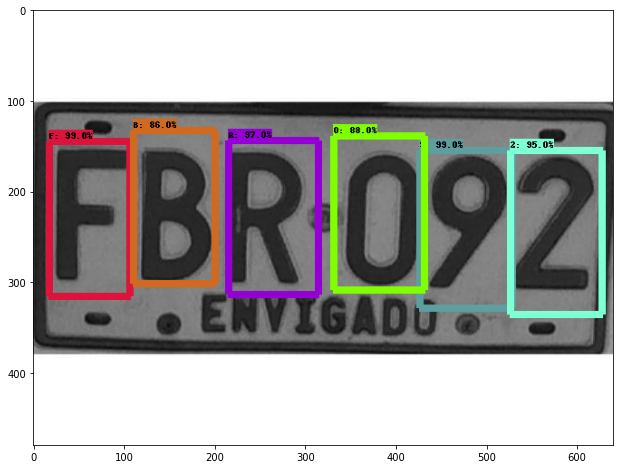
\includegraphics[width=0.4\linewidth]{imagenes/caracteres detectados/nuevo entrenamiento/1.png}
\caption{Placa 15}
\label{fig:caracteres detectados p17}
\end{figure}

\begin{table}[H]
    \centering
    \resizebox{\textwidth}{!}{
    \begin{tabular}{||c|c|c||}
    \hline \hline
         Caracter Placa & Caracter detectado & Porcentaje de reconocimiento \\  \hline \hline
         Letra F & Letra F & 99\%  \\ \cline{1-3}
         Letra B & Letra B & 86\%  \\ \cline{1-3}
         Letra R & Letra R & 97\%  \\ \cline{1-3}
         Número 0 & Número 0 & 88\%  \\ \cline{1-3}
         Número 9 & Número 9 & 99\%  \\ \cline{1-3}
         Número 2 & Número 2 & 95\% \\ \hline
         \hline
         \end{tabular}
    }
    \caption{Detección de caracteres con porcentajes de acierto placa 15}
    \label{tab:p17}
\end{table}


% PLACA 18------------

\begin{figure}[H]
\centering
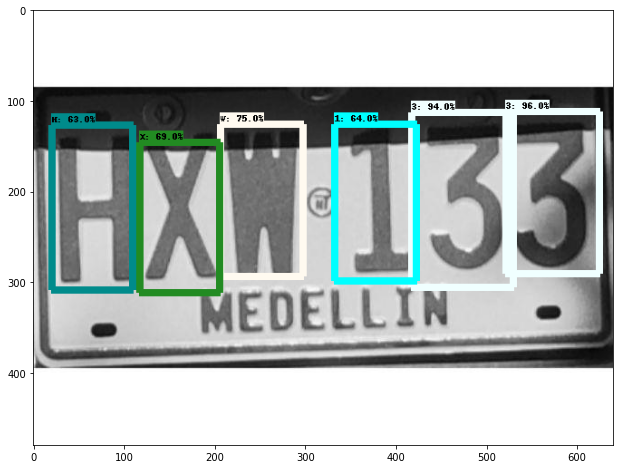
\includegraphics[width=0.4\linewidth]{imagenes/caracteres detectados/nuevo entrenamiento/6.png}
\caption{Placa 16}
\label{fig:caracteres detectados p18}
\end{figure}

\begin{table}[H]
    \centering
    \resizebox{\textwidth}{!}{
    \begin{tabular}{||c|c|c||}
    \hline \hline
         Caracter Placa & Caracter detectado & Porcentaje de reconocimiento \\  \hline \hline
         Letra H & Letra H & 63\%  \\ \cline{1-3}
         Letra X & Letra X & 69\%  \\ \cline{1-3}
         Letra W & Letra W & 75\%  \\ \cline{1-3}
         Número 1 & Número 1 & 64\%  \\ \cline{1-3}
         Número 3 & Número 3 & 94\% \\ \cline{1-3}
         Número 3 & Número 3 & 96\% \\ \hline
         \hline
         \end{tabular}
    }
    \caption{Detección de caracteres con porcentajes de acierto placa 16}
    \label{tab:p18}
\end{table}

%PLACA 17
\begin{figure}[H]
\centering
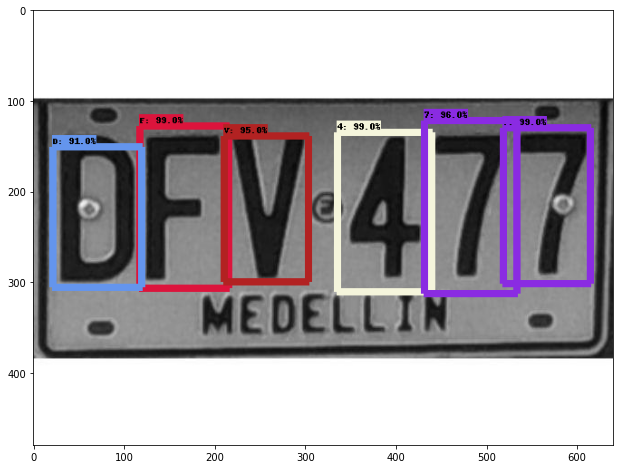
\includegraphics[width=0.4\linewidth]{imagenes/caracteres detectados/nuevo entrenamiento/10.png}
\caption{Placa 17}
\label{fig:caracteres detectados p19}
\end{figure}



\begin{table}[H]
    \centering
    \resizebox{\textwidth}{!}{
    \begin{tabular}{||c|c|c||}
    \hline \hline
         Caracter Placa & Caracter detectado & Porcentaje de reconocimiento \\  \hline \hline
         Letra D & Letra D & 91\%  \\ \cline{1-3}
         Letra F & Letra F & 99\%  \\ \cline{1-3}
         Letra V & Letra V & 95\%  \\ \cline{1-3}
         Número 4 & Número 4 & 99\%  \\ \cline{1-3}
         Número 7 & Número 7 & 96\%  \\ \cline{1-3}
         Número 7 & Número 7 & 99\% \\ \hline
         \hline
         \end{tabular}
    }
    \caption{Detección de caracteres con porcentajes de acierto placa 17}
    \label{tab:p19}
\end{table}


% PLACA 18

\begin{figure}[H]
\centering
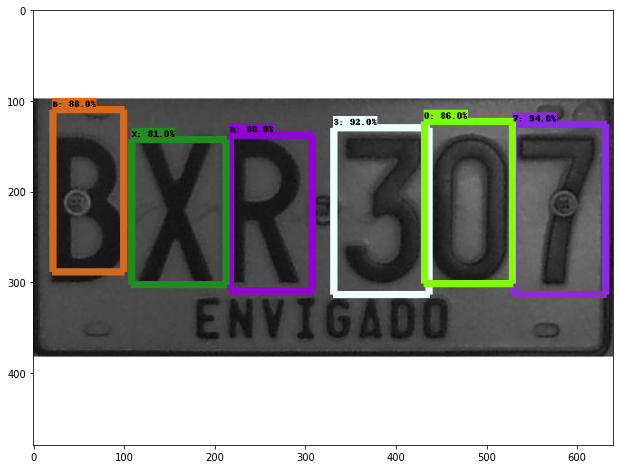
\includegraphics[width=0.4\linewidth]{imagenes/caracteres detectados/nuevo entrenamiento/16.png}
\caption{Placa 18}
\label{fig:caracteres detectados p21}
\end{figure}

\begin{table}[H]
    \centering
    \resizebox{\textwidth}{!}{
    \begin{tabular}{||c|c|c||}
    \hline \hline
         Caracter Placa & Caracter detectado & Porcentaje de reconocimiento  \\  \hline \hline
         Letra B & Letra B & 88\%  \\ \cline{1-3}
         Letra X & Letra X & 81\%\\ \cline{1-3}
         Letra R & Letra R & 88\%  \\ \cline{1-3}
         Número 3 & Número 3 & 92\%  \\ \cline{1-3}
         Número 0 & Número 0 & 86\%  \\ \cline{1-3}
         Número 7 & Número 7 & 94\% \\ \hline
         \hline
         \end{tabular}
    }
    \caption{Detección de caracteres con porcentajes de acierto placa 18}
    \label{tab:p21}
\end{table}



% PLACA 19
\begin{figure}[H]
\centering
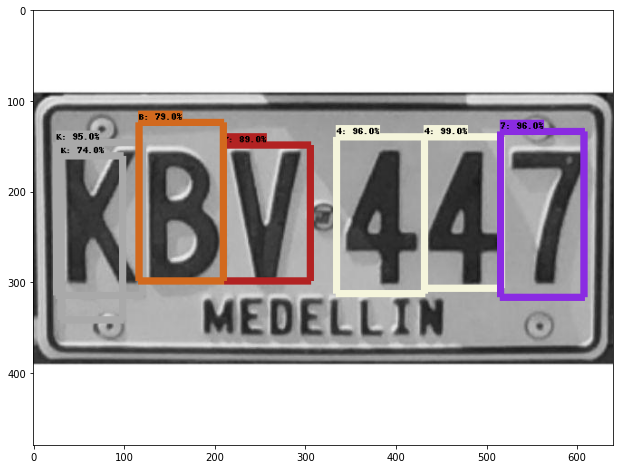
\includegraphics[width=0.4\linewidth]{imagenes/caracteres detectados/nuevo entrenamiento/19.png}
\caption{Placa 19}
\label{fig:caracteres detectados p23}
\end{figure}



\begin{table}[H]
    \centering
    \resizebox{\textwidth}{!}{
    \begin{tabular}{||c|c|c||}
    \hline \hline
         Caracter Placa & Caracter detectado & Porcentaje de reconocimiento \\  \hline \hline
         Letra K & Letra K & 95\%  \\ \cline{1-3}
         Letra B & Letra B & 79\%  \\ \cline{1-3}
         Letra V & Letra V & 89\%  \\ \cline{1-3}
         Número 4 & Número 4 & 96\%  \\ \cline{1-3}
         Número 4 & Número 4 & 99\%  \\ \cline{1-3}
         Número 7 & Número 7 & 96\% \\ \hline
         \hline
         \end{tabular}
    }
    \caption{Detección de caracteres con porcentajes de acierto placa 19}
    \label{tab:p23}
\end{table}

% PLACA 20

\begin{figure}[H]
\centering
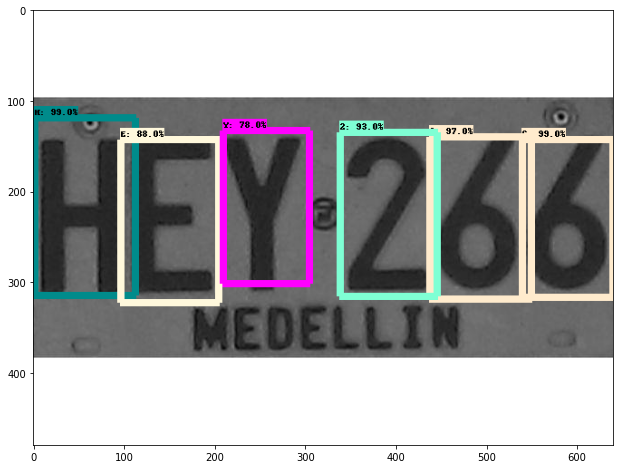
\includegraphics[width=0.4\linewidth]{imagenes/caracteres detectados/nuevo entrenamiento/22.png}
\caption{Placa 20}
\label{fig:caracteres detectados p24}
\end{figure}

\begin{table}[H]
    \centering
    \resizebox{\textwidth}{!}{
    \begin{tabular}{||c|c|c||}
    \hline \hline
         Caracter Placa & Caracter detectado & Porcentaje de reconocimiento\\  \hline \hline
         Letra H & Letra H & 99\%  \\ \cline{1-3}
         Letra E & Letra E & 88\%  \\ \cline{1-3}
         Letra Y & Letra Y & 78\%  \\ \cline{1-3}
         Número 2 & Número 2 & 93\%  \\ \cline{1-3}
         Número 6 & Número 6 & 97\%  \\ \cline{1-3}
         Número 6 & Número 6 & 99\% \\ \hline
         \hline
         \end{tabular}
    }
    \caption{Detección de caracteres con porcentajes de acierto placa 20}
    \label{tab:p24}
\end{table}


% PLACA 21

\begin{figure}[H]
\centering
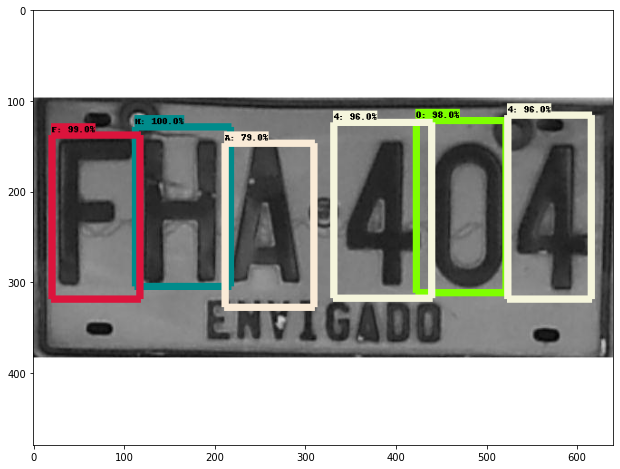
\includegraphics[width=0.4\linewidth]{imagenes/caracteres detectados/nuevo entrenamiento/27.png}
\caption{Placa 21}
\label{fig:caracteres detectados p26}
\end{figure}

\begin{table}[H]
    \centering
    \resizebox{\textwidth}{!}{
    \begin{tabular}{||c|c|c||}
    \hline \hline
         Caracter Placa & Caracter detectado & Porcentaje de reconocimiento  \\  \hline \hline
         Letra F & Letra F & 99\%  \\ \cline{1-3}
         Letra H & Letra H & 100\%  \\ \cline{1-3}
         Letra A & Letra A & 79\%  \\ \cline{1-3}
         Número 4 & Número 4 & 96\%  \\ \cline{1-3}
         Número 0 & Número 0 & 98\%  \\ \cline{1-3}
         Número 4 & Número 4 & 96\% \\ \hline
         \hline
         \end{tabular}
    }
    \caption{Detección de caracteres con porcentajes de acierto placa 21}
    \label{tab:p26}
\end{table}

% PLACA 22

\begin{figure}[H]
\centering
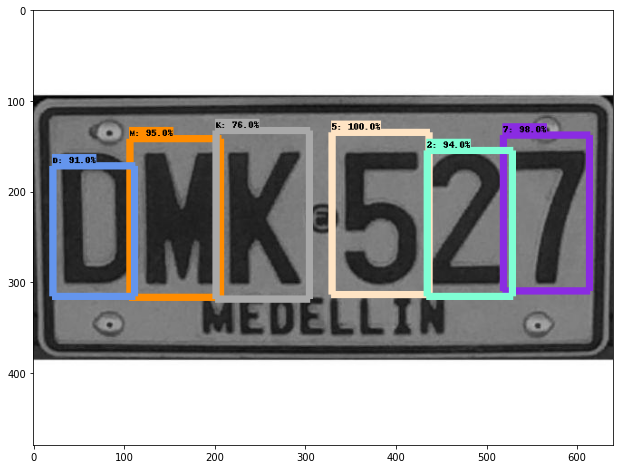
\includegraphics[width=0.4\linewidth]{imagenes/caracteres detectados/nuevo entrenamiento/31.png}
\caption{Placa 22}
\label{fig:caracteres detectados p27}
\end{figure}

\begin{table}[H]
    \centering
    \resizebox{\textwidth}{!}{
    \begin{tabular}{||c|c|c||}
    \hline \hline
         Caracter Placa & Caracter detectado & Porcentaje de reconocimiento \\  \hline \hline
         Letra D & Letra D & 91\%  \\ \cline{1-3}
         Letra M & Letra M & 95\%  \\ \cline{1-3}
         Letra K & Letra K & 76\%  \\ \cline{1-3}
         Número 5 & Número 5 & 100\%  \\ \cline{1-3}
         Número 2 & Número 2 & 94\% \\ \cline{1-3}
         Número 7 & Número 7 & 98\% \\ \hline
         \hline
         \end{tabular}
    }
    \caption{Detección de caracteres con porcentajes de acierto placa 22}
    \label{tab:p27}
\end{table}



% PLACA 23

\begin{figure}[H]
\centering
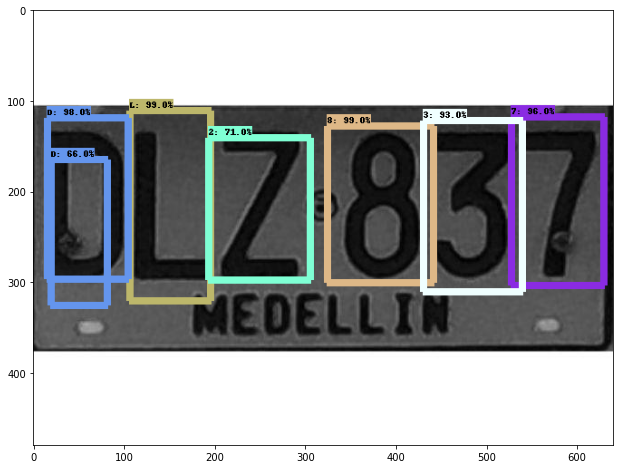
\includegraphics[width=0.4\linewidth]{imagenes/caracteres detectados/nuevo entrenamiento/7.png}
\caption{Placa 23}
\label{fig:caracteres detectados p29}
\end{figure}

\begin{table}[H]
    \centering
    \resizebox{\textwidth}{!}{
    \begin{tabular}{||c|c|c||}
    \hline \hline
         Caracter Placa & Caracter detectado & Porcentaje de reconocimiento \\  \hline \hline
         Letra D & Letra D & 98\%  \\ \cline{1-3}
         Letra L & Letra L & 99\%  \\ \cline{1-3}
         Letra Z & Letra Z & 71\%  \\ \cline{1-3}
         Número 8 & Número 8 & 99\% \\ \cline{1-3}
         Número 3 & Número 3 & 93\%  \\ \cline{1-3}
         Número 7 & Número 7 & 96\% \\ \hline
         \hline
         \end{tabular}
    }
    \caption{Detección de caracteres con porcentajes de acierto placa 23}
    \label{tab:p29}
\end{table}

% PLACA 30

\begin{figure}[H]
\centering
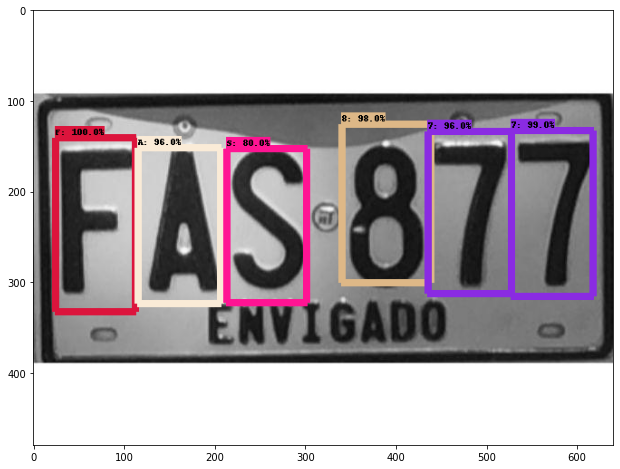
\includegraphics[width=0.4\linewidth]{imagenes/caracteres detectados/nuevo entrenamiento/8.png}
\caption{Placa 24}
\label{fig:caracteres detectados p30}
\end{figure}

\begin{table}[H]
    \centering
    \resizebox{\textwidth}{!}{
    \begin{tabular}{||c|c|c||}
    \hline \hline
         Caracter Placa & Caracter detectado & Porcentaje de reconocimiento  \\  \hline \hline
         Letra F & Letra F & 100\%   \\ \cline{1-3}
         Letra A & Letra A & 96\% \\ \cline{1-3}
         Letra S & Letra S & 80\% \\ \cline{1-3}
         Número 8 & Número 8 & 98\% \\ \cline{1-3}
         Número 7 & Número 7 & 96\% \\ \cline{1-3}
         Número 7 & Número 7 & 99\% \\ \hline
         \hline
         \end{tabular}
    }
    \caption{Detección de caracteres con porcentajes de acierto placa 24}
    \label{tab:p30}
\end{table}



% PLACA 32

\begin{figure}[H]
\centering
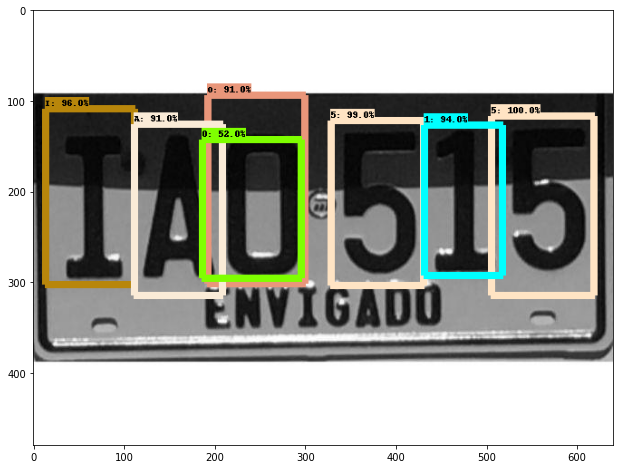
\includegraphics[width=0.4\linewidth]{imagenes/caracteres detectados/nuevo entrenamiento/15.png}
\caption{Placa 25}
\label{fig:caracteres detectados p32}
\end{figure}

\begin{table}[H]
    \centering
    \resizebox{\textwidth}{!}{
    \begin{tabular}{||c|c|c||}
    \hline \hline
         Caracter Placa & Caracter detectado & Porcentaje de reconocimiento \\  \hline \hline
         Letra I & Letra I & 96\%  \\ \cline{1-3}
         Letra A & Letra A & 91\% \\ \cline{1-3}
         Letra O & Letra O & 91\%  \\ \cline{1-3}
         Número 5 & Número 5 & 99\%  \\ \cline{1-3}
         Número 1 & Número 1 & 94\%  \\ \cline{1-3}
         Número 5 & Número 5 & 100\% \\ \hline
         \hline
         \end{tabular}
    }
    \caption{Detección de caracteres con porcentajes de acierto placa 25}
    \label{tab:p32}
\end{table}

\subsection*{Análisis}

Se puede observar que en 25 imágenes de 32 se detectaron todos los caracteres y todos fueron reconocidos correctamente con un porcentaje relativamente alto. Este es un buen resultado a pesar de que no se entrenó con una base de datos no muy extensa, variable y equilibrada.

%===================================
\subsection{Placas con caracteres no reconocidos o reconocidos con bajo porcentaje}

% PLACA 26

\begin{figure}[H]
\centering
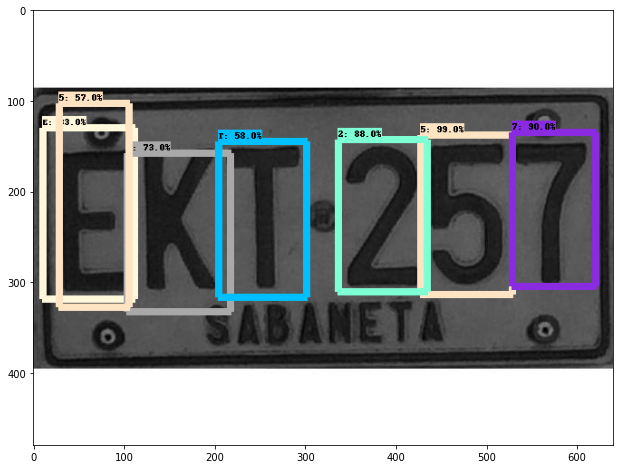
\includegraphics[width=0.4\linewidth]{imagenes/caracteres detectados/nuevo entrenamiento/11.png}
\caption{Placa 26}
\label{fig:caracteres detectados p31}
\end{figure}

\begin{table}[H]
    \centering
    \resizebox{\textwidth}{!}{
    \begin{tabular}{||c|c|c||}
    \hline \hline
         Caracter Placa & Caracter detectado & Porcentaje de reconocimiento  \\  \hline \hline
         Letra E & Letra E & 93\%  \\ \cline{1-3}
         Letra K & Letra K & 73\%  \\ \cline{1-3}
         Letra T & Letra T & \textcolor{red}{58\%}  \\ \cline{1-3}
         Número 2 & Número 2 & 88\%  \\ \cline{1-3}
         Número 5 & Número 5 & 99\%  \\ \cline{1-3}
         Número 7 & Número 7 & 90\% \\ \hline
         \hline
         \end{tabular}
    }
    \caption{Detección de caracteres con porcentajes de acierto placa 26}
    \label{tab:p31}
\end{table}

% PLACA 27

\begin{figure}[H]
\centering
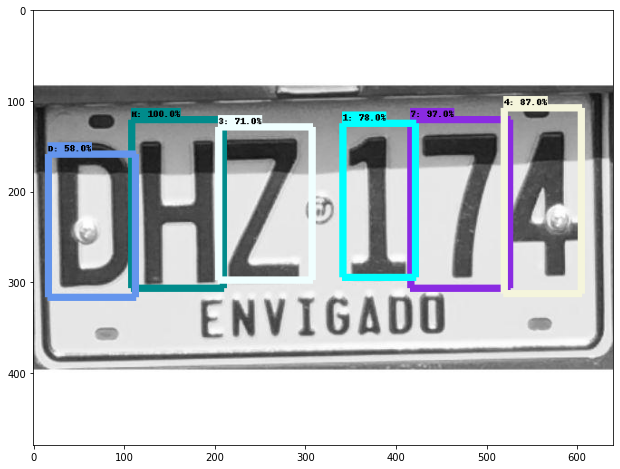
\includegraphics[width=0.4\linewidth]{imagenes/caracteres detectados/nuevo entrenamiento/32.png}
\caption{Placa 27}
\label{fig:caracteres detectados p28}
\end{figure}

\begin{table}[H]
    \centering
    \resizebox{\textwidth}{!}{
    \begin{tabular}{||c|c|c||}
    \hline \hline
         Caracter Placa & Caracter detectado & Porcentaje de reconocimiento  \\  \hline \hline
         Letra D & Letra D & \textcolor{red}{58\%} \\ \cline{1-3}
         Letra H & Letra H & 100\%  \\ \cline{1-3}
         Letra Z & Letra Z & 71\% \\ \cline{1-3}
         Número 1 & Número 1 & 78\% \\ \cline{1-3}
         Número 7 & Número 7 & 97\% \\ \cline{1-3}
         Número 4 & Número 4 & 87\% \\ \hline
         \hline
         \end{tabular}
    }
    \caption{Detección de caracteres con porcentajes de acierto placa 27}
    \label{tab:p28}
\end{table}

%PLACA 28

\begin{figure}[H]
\centering
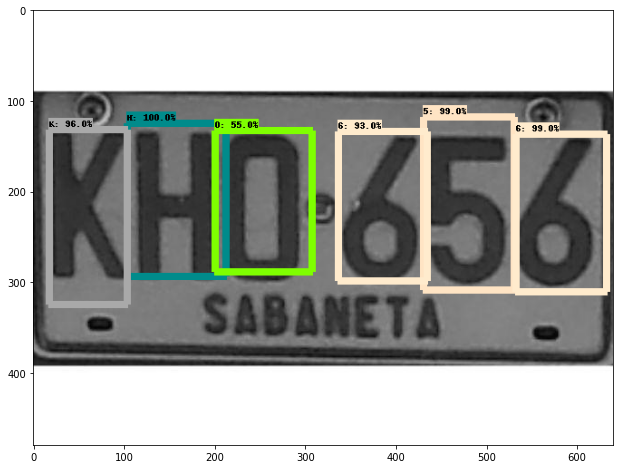
\includegraphics[width=0.4\linewidth]{imagenes/caracteres detectados/nuevo entrenamiento/17.png}
\caption{Placa 28}
\label{fig:caracteres detectados p22}
\end{figure}

\begin{table}[H]
    \centering
    \resizebox{\textwidth}{!}{
    \begin{tabular}{||c|c|c||}
    \hline \hline
         Caracter Placa & Caracter detectado & Porcentaje de reconocimiento  \\  \hline \hline
         Letra K & Letra K & 96\%  \\ \cline{1-3}
         Letra H & Letra H & 100\%  \\ \cline{1-3}
         Letra D & \textcolor{red}{Número 0} & \textcolor{red}{55\%}  \\ \cline{1-3}
         Número 6 & Número 6 & 93\%  \\ \cline{1-3}
         Número 5 & Número 5 & 99\%  \\ \cline{1-3}
         Número 6 & Número 6 & 99\% \\ \hline
         \hline
         \end{tabular}
    }
    \caption{Detección de caracteres con porcentajes de acierto placa 28}
    \label{tab:p22}
\end{table}


% PLACA 29

\begin{figure}[H]
\centering
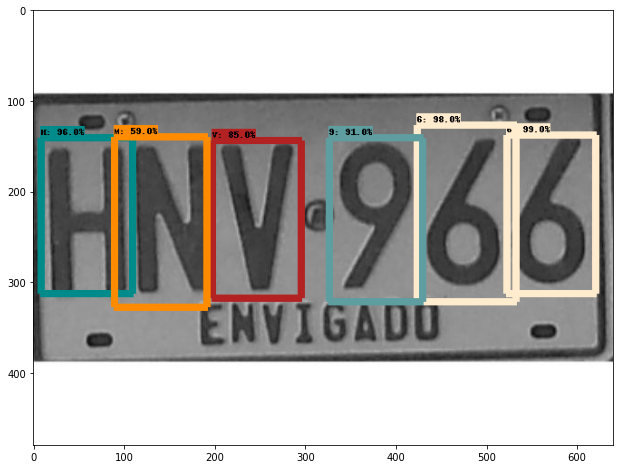
\includegraphics[width=0.4\linewidth]{imagenes/caracteres detectados/nuevo entrenamiento/14.png}
\caption{Placa 29}
\label{fig:caracteres detectados p20}
\end{figure}

\begin{table}[H]
    \centering
    \resizebox{\textwidth}{!}{
    \begin{tabular}{||c|c|c||}
    \hline \hline
         Caracter Placa & Caracter detectado & Porcentaje de reconocimiento  \\  \hline \hline
         Letra H & Letra H & 96\% \\ \cline{1-3}
         Letra N & Letra N & \textcolor{red}{59\%} \\ \cline{1-3}
         Letra V & Letra V & 85\%  \\ \cline{1-3}
         Número 9 & Número 9 & 91\%  \\ \cline{1-3}
         Número 6 & Número 6 & 98\%  \\ \cline{1-3}
         Número 6 & Número 6 & 99\% \\ \hline
         \hline
         \end{tabular}
    }
    \caption{Detección de caracteres con porcentajes de acierto placa 29}
    \label{tab:p20}
\end{table}

% PLACA 30-----------
\begin{figure}[H]
\centering
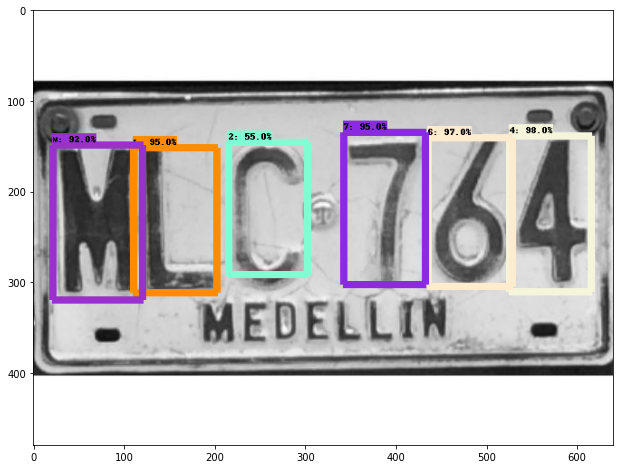
\includegraphics[width=0.4\linewidth]{imagenes/caracteres detectados/12.png}
\caption{Placa 30}
\label{fig:caracteres detectados p12}
\end{figure}

\begin{table}[H]
    \centering
    \resizebox{\textwidth}{!}{
    \begin{tabular}{||c|c|c||}
    \hline \hline
         Caracter Placa & Caracter detectado & Porcentaje de reconocimiento l \\  \hline \hline
         Letra M & Letra M & 92\%   \\ \cline{1-3}
         Letra L & Letra L & 95\%  \\ \cline{1-3}
         Letra C & Letra C & \textcolor{red}{55\%}  \\ \cline{1-3}
         Número 7 & Número 7 & 95\% \\ \cline{1-3}
         Número 6 & Número 6 & 97\%  \\ \cline{1-3}
         Número 4 & Número 4 & 98\% \\ \hline
         \hline
         \end{tabular}
    }
    \caption{Detección de caracteres con porcentajes de acierto placa 30}
    \label{tab:p12}
\end{table}


% PLACA 31----------
\begin{figure}[H]
\centering
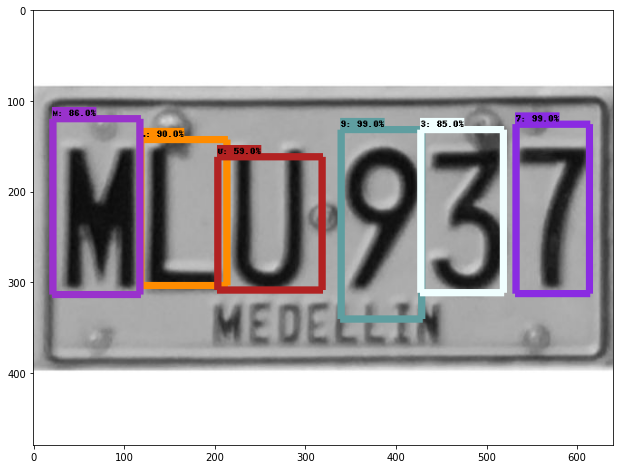
\includegraphics[width=0.4\linewidth]{imagenes/caracteres detectados/4.png}
\caption{Placa 31}
\label{fig:caracteres detectados p4}
\end{figure}

\begin{table}[H]
    \centering
    \resizebox{\textwidth}{!}{
    \begin{tabular}{||c|c|c||}
    \hline \hline
         Caracter Placa & Caracter detectado & Porcentaje de reconocimiento
         \\  \hline \hline
         Letra M & Letra M & 99\%  \\ \cline{1-3}
         Letra L & Letra L & 90\%  \\ \cline{1-3}
         Letra U & Letra U & \textcolor{red}{59\%} \\ \cline{1-3}
         Número 9 & Número 9 & 99\% \\ \cline{1-3}
         Número 3 & Número 3 & 85\% \\ \cline{1-3}
         Número 7 & Número 7 & 99\% \\ \hline \hline
    \end{tabular}
    }
    \caption{Detección de caracteres con porcentajes de acierto placa 31}
    \label{tab:p4}
\end{table}

% PLACA 32

\begin{figure}[H]
\centering
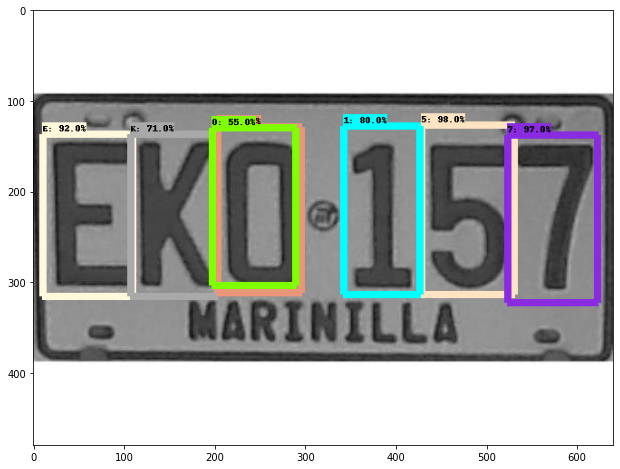
\includegraphics[width=0.4\linewidth]{imagenes/caracteres detectados/nuevo entrenamiento/24.png}
\caption{Placa 32}
\label{fig:caracteres detectados p25}
\end{figure}

\begin{table}[H]
    \centering
    \resizebox{\textwidth}{!}{
    \begin{tabular}{||c|c|c||}
    \hline \hline
         Caracter Placa & Caracter detectado & Porcentaje de reconocimiento \\  \hline \hline
         Letra E & Letra E & 92\% \\ \cline{1-3}
         Letra K & Letra K & 71\%  \\ \cline{1-3}
         Letra O & \textcolor{red}{Número 0} & \textcolor{red}{55\%}  \\ \cline{1-3}
         Número 1 & Número 1 & 80\%  \\ \cline{1-3}
         Número 5 & Número 5 & 98\%  \\ \cline{1-3}
         Número 7 & Número 7 & 97\% \\ \hline
         \hline
         \end{tabular}
    }
    \caption{Detección de caracteres con porcentajes de acierto placa 32}
    \label{tab:25}
\end{table}

\subsection*{Análisis}

Observamos que en algunas placas las letras U, N, C, T y D son reconocidas correctamente pero con un bajo porcentaje.  También, se observa en otras placas que las letras D y O no son reconocidas, estas son confundidas con el número 0. Esto se debe principalmente a la poca frecuencia que tienen estos caracteres en la base de datos \textit{CharsBoxPlateCol} usada para el entrenamiento (ver sección \ref{fig:frecuencia3}). La confusión de las letras D y O con el cero puede ser debido a que son caracteres muy similares y prevalece en el reconocimiento el caracter que haya sido mejor entrenado, es decir, el que tenga mayor frecuencia y variablilidad (el cero en este caso).

%======================================
\begin{tcolorbox}
[colback=blue!5!white,colframe=blue!45!black,fonttitle=\bfseries,title=Conclusión]

A pesar de que no se entrenó con una base de datos no muy extensa, con la transferencia de aprendizaje usando la técnica de detección de objetos se obtiene resultados prometedores.
El rendimiento se puede mejorar si se realiza el entrenamiento con una base de datos muy bien equilibrada y con suficiente variabilidad. 

\end{tcolorbox}\\




\begin{comment}
    
\section{Rendimiento Base de datos \textit{CharsBoxPlateCol} }

Para medir el rendimiento del algoritmo de detección de caracteres se usan las métricas de detección COCO, las cuales muestran las medidas de mAP (mean Average Precisión) y AR (Average Recall).

\begin{table}[H]
    \centering
    \resizebox{\textwidth}{!}{
       \begin{tabular}{||c|c|p{3cm}|c|c|c|c|c||}
        \hline \hline
        \multicolumn{8}{||c||}{\verb"PRECISION"}\\ \hline \hline
         Tiempo de evaluación conjunto de datos & FASTER R-CNN & Promedio precision/maP & precision(pequeno)& precision(mediano) & precision(grande) & precision IoU = 0.5 & precision IoU = 0.75   \\ \hline
         0.06 segundos & Inception v2 & 0.733 & -1 & -1 & 0.733 & 1 & 1\\ \hline \hline
         
    \end{tabular}
    }
    \caption{Precision después del entrenamiento con la base de datos  \textit{CharsBoxPlateCol}}
    \label{tab:precision CharsBoxPlateCol}
\end{table}


\begin{table}[H]
    \centering
    \resizebox{\textwidth}{!}{
       \begin{tabular}{||c|c|p{3cm}|c|c|c|c|c||}
        \hline \hline
        \multicolumn{8}{||c||}{\verb"RECALL"}\\ \hline \hline
         Tiempo de evaluación conjunto de datos & FASTER R-CNN & Promedio Recall/maP & Recall(pequeno)& Recall(mediano) & Recall(grande) & Recall AR@10 & Recall AR@100   \\ \hline
        0.06 segundos & Inception v2 & 0.733 & -1 & -1 & 0.733 & 0.733 & 0.733\\ \hline \hline
         
    \end{tabular}
    }
    \caption{Recall después del entrenamiento con la base de datos  \textit{CharsBoxPlateCol}}
    \label{tab:Recall CharsBoxPlateCol}
\end{table}


\section{Resultado usando la base de datos \textit{CharsBoxPlateCol} con aumento de datos}

Para medir el rendimiento del algoritmo de detección de caracteres se usan las métricas de detección COCO, las cuales muestran las medidas de mAP (mean Average Precision) y AR (Average Recall).

\begin{table}[H]
    \centering
    \resizebox{\textwidth}{!}{
       \begin{tabular}{||c|c|p{3cm}|c|c|c|c|c||}
        \hline \hline
        \multicolumn{8}{||c||}{\verb"PRECISION"}\\ \hline \hline
         Tiempo de evaluación conjunto de datos & FASTER R-CNN & Promedio precision/maP & precision(pequeño)& precision(mediano) & precision(grande) & precision IoU = 0.5 & precision IoU = 0.75   \\ \hline
         9.5 segundos & Inception v2 & 0.557 & -1 & 0.559 & 0.589 & 0.872 & 0.665\\ \hline \hline
    \end{tabular}
    }
    \caption{Precision después del entrenamiento con la base de datos  \textit{CharsBoxPlateCol} con data augmentation}
    \label{tab:precision con con data augmentation}
\end{table}


\begin{table}[H]
    \centering
    \resizebox{\textwidth}{!}{
       \begin{tabular}{||c|p{3cm}|c|p{3cm}|c|c|c|c|c||}
        \hline \hline
        \multicolumn{8}{||c||}{\verb"RECALL"}\\ \hline \hline
         Tiempo de evaluación conjunto de datos & FASTER R-CNN & Promedio Recall/maP & Recall(pequeño)& Recall(mediano) & Recall(grande) & Recall AR@10 & Recall AR@100   \\ \hline
         9.5 segundos &Inception v2 & 0.625 & -1 & 0.699 & 0.684 & 0.685 & 0.685\\ \hline \hline
         
    \end{tabular}
    }
    \caption{Recall después del entrenamiento con la base de datos  \textit{CharsBoxPlateCol} con data augmentation}
    \label{tab:Recall con data augmentation}
\end{table}
\end{comment}

\section{Comparación del Modelo 1 con el Modelo 2}

Hemos creado dos sistemas de reconocimiento de caracteres en placas colombianas. Uno a partir de una Red Neuronal Convolucional para clasificación construida desde cero (Modelo 1) y otro usando transferencia de aprendizaje a partir de una red pre-entrenada para detección de objetos (Modelo 2). Para realizar una comparación se han evaluado los dos sistemas sobre un mismo conjunto de 32 placas, las cuales no han participado en el entrenamiento. Se considera que una placa no ha sido reconocida si ha fallado en reconocer, por lo menos, uno de sus caracteres.


{\centering
\begin{table}[H]
    \begin{center}
    \centering
    \resizebox{0.7\textwidth}{!}{
    %\begin{tabular}{||p{1.5cm}|p{2cm}|p{3cm}|p{3cm}|p{3cm}|p{3cm}||}
    \begin{tabular}{||c|c||c|c||c|c||}
    \hline \hline
    %\multicolumn{1}{|c|}{\multirow{2}{*}{\textbf{\begin{tabular}[c]{@{}c@{}}\\ \end{tabular}}}} 
  
     & & \multicolumn{2}{|c||}{Modelo 1} & \multicolumn{2}{|c||}{Modelo 2}\\ \hline
        & Placa de entrada & Caracteres Reconocidos & Reconoce la placa & Caracter reconocido  & Reconoce la placa \\ \hline \hline
        
        1 & MVW 162 & MVW 162 & SI & MVW 162  & SI \\ \hline
         2 & MLF 905 & MLF 905 & NO & MLF 905 & SI\\ \hline
         3 & BXR 307 & BXR 307 &  NO & BXR 307 & SI \\ \hline
         4 & MLU 937 & ML\textcolor{red}{O} 937 & \textcolor{red}{NO} & MLU 937 & SI \\ \hline
         5 & MOL 514 & MOL 514 & NO & MOL 514 & SI \\ \hline
         6 & KHK 343 & KHK 343 & NO & KHK 343 & SI \\ \hline
         7 & MOM 597 & MOM 597 & SI & MOM 597 & SI \\ \hline
         8 & DEU 087 & DE\textcolor{red}{U} 087 & \textcolor{red}{NO} & DEU 087 & SI \\ \hline
         9 & HGW 532 & H\textcolor{red}{CV} 532 & \textcolor{red}{NO} & HGW 532 & SI \\ \hline
         10 & EKO 814 & EKO 814 & SI & EKO 814 & SI \\ \hline
         11 & MVV 827 & MVV 827 & SI & MVV 827 & SI \\ \hline
         12 & MLC 764 & MLC 764 & SI  & MLC 764 & SI \\ \hline
         13 & HXT 577 & HXT 577 & SI & HXT 577 & SI \\ \hline
         14 & HXX 192 & HXX 192 & SI & HXX 192 & SI \\ \hline
         15 & FGR 112 & FGR 112 & SI & FGR 112 & SI \\ \hline
         16 & BLF 275 & BLF 275 & SI & BLF 275 & SI \\ \hline
         17 & FBR 092 & FBR 092 & SI & FBR 092 & SI \\ \hline
         18 & HXW 133 & HXW 133 & SI & HXW 133 & SI \\ \hline
         19 & DFV 477 & D\textcolor{red}{F}V 477 & \textcolor{red}{NO} & DFV 477 & SI \\ \hline
         20 & HNV 966 & HNV 966 & SI & HNV 966 & SI \\ \hline
         21 & BXR 307 & BXR 307 & SI & BXR 307 & SI \\ \hline
         22 & KHD 656 & KHD 656 & SI & KH\textcolor{red}{O} 656 & \textcolor{red}{NO} \\ \hline
         23 & KBV 447 & KBV 447 & SI & KBV 447 & SI \\ \hline
         24 & HEY 266 & HEY 266 & SI & HEY 266 &  SI \\ \hline
         25 & EKO 157 & EKO 157 & SI & EK\textcolor{red}{0} 157 & \textcolor{red}{NO} \\ \hline
         26 & FHA 404 &  FHA 404 & SI &  FHA 404 & SI \\ \hline
         28 & DMK 527 & DMK 527 & SI & DMK 527 & SI \\ \hline
         29 & DHZ 174 & DHZ 174 & SI & DHZ 174 & SI \\ \hline
         30 & DLZ 837 & D\textcolor{red}{I}Z 837 &  \textcolor{red}{NO} & DL\textcolor{red}{2} 837 & \textcolor{red}{NO} \\ \hline
         31 & FAS 877 & FAS 877 & SI & FAS 877 & SI \\ \hline
         32 & EKT 257 & EK\textcolor{red}{F} 257 & \textcolor{red}{NO} & EKT 257 & SI \\ \hline \hline 
    \end{tabular}
    }
    \end{center}
    \caption{Reconocimiento de placas de acuerdo a cada sistema}
    \label{tab:comparacion}
\end{table}}

En la taba \ref{tab:comparacion} se realiza un resumen de las placas reconocidas tanto por el modelo 1 como por el modelo 2. Los caracteres en rojo son los que el modelo falló. Con el modelo 1 se logró un 81,25\% de reconocimiento en relación con el total de las 32 placas y con el modelo 2 se logro un 96,25\%.

El modelo 2 presenta resultados prometedores, ya que a pesar de ser entrenada con una base de datos no muy equilibrada ni con mucha variabilidad los resultados han sido mejores que el obtenido con el modelo 1, el cual fue entrenado con una base de datos más equilibrada y variable.

Por otro lado, el sistema de reconocimiento implementado usando el Modelo 2 tiene algunas ventajas respecto al sistema implementado usando el modelo 1; ya que, aunque en los dos se tiene que segmentar la placa entera desde la imagen del automovil, en el sistema que usa en Modelo 2 no se tiene que realizar nuevamente otra segmentación para extraer cada caracter de la placa. Mientras que, en el sistema que usa el Modelo 1, se tiene que volver a segmentar cada caracter desde la placa para ser reconocido. Además, usando detección de objetos el sistema de reconocimiento se puede aplicar para otros formatos. Por ejemplo, para cualquier cantidad de caracteres en una placa o la forma como estén arreglados (en filas o columnas, etc). Por ejemplo, en la figura \ref{fig:5caracteres} se muestra el resultado del sistema para una placa con 5 caracteres. 

\begin{figure}[h]
\centering
  {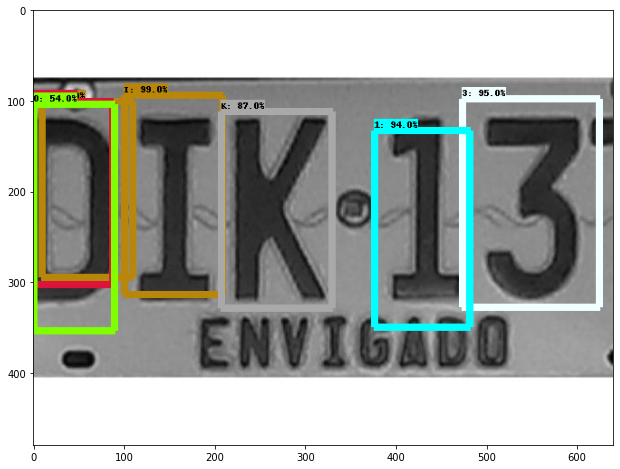
\includegraphics[width=0.4\textwidth]{imagenes/caracteres detectados/nuevo entrenamiento/5.png}}
    \caption{Resultado de la detección de 5 caracteres por medio de una Faster R-CNN }
    \label{fig:5caracteres}  
\end{figure}

